\documentclass[a4paper,12pt]{article}
\usepackage{WSEIRap} 
\usepackage{pgf-umlcd}
\renewcommand{\titleLab}{Inteligentny Asystent Śniadań}
\renewcommand{\Author}{Mateusz Wnuk}
\renewcommand{\Students}{~}
\renewcommand{\lab}{Zarządznie projektami IT}
\renewcommand{\groupLab}{Gr-6}
\renewcommand{\Date}{1-10-2024}
\renewcommand{\Rodzaj}{Raport}

\begin{document}
\RapPage

\section{Inteligentny Asystent Śniadań}\label{sec:inteligentny-asystent-sniadan}

\subsection{Opis Projektu}\label{subsec:opis-projektu}

Inteligentny Asystent Śniadań to nowoczesna aplikacja mobilna stworzona z myślą o ułatwieniu codziennych porannych rutyn.
Główne cele projektu to:
\begin{enumerate}
    \item \textbf{Automatyzacja Procesu Przygotowywania Śniadań:} Aplikacja pomoże użytkownikom tworzyć spersonalizowane plany śniadaniowe, uwzględniając ich preferencje dietetyczne, dostępne składniki oraz czas, jaki mogą poświęcić na przygotowanie posiłku.
    \item \textbf{Zarządzanie Zasobami Kuchennymi:} Asystent będzie monitorował stan zapasów kuchennych i sugerował zakupy niezbędnych produktów.
    \item \textbf{Porady Żywieniowe i Zdrowotne:} Aplikacja dostarczy użytkownikom cennych informacji na temat wartości odżywczych posiłków, sugerując zdrowe zamienniki oraz optymalne porcje.
    \item \textbf{Integracja z Urządzeniami IoT:} Asystent będzie mógł współpracować z inteligentnymi urządzeniami kuchennymi, takimi jak inteligentne lodówki, kuchenki czy blendery, aby jeszcze bardziej usprawnić proces przygotowywania posiłków.
    \item \textbf{Interaktywne Przepisy:} Użytkownicy będą mieli dostęp do bazy interaktywnych przepisów, które będą dostosowywane na bieżąco w zależności od dostępnych składników oraz preferencji dietetycznych.
    \item \textbf{Automatyczne Przygotowywanie Śniadań:} Asystent będzie mógł sterować urządzeniami kuchennymi, aby automatycznie przygotować śniadanie na zadaną godzinę.
\end{enumerate}

\subsection{Wymagania Projektowe}\label{subsec:wymagania-projektowe}

\subsubsection{Funkcjonalność}
\begin{itemize}
    \item \textbf{Tworzenie Planów Śniadaniowych:}
    \begin{itemize}
        \item Personalizacja na podstawie preferencji dietetycznych użytkownika.
        \item Uwzględnianie dostępnych składników.
        \item Opcje dla osób z ograniczeniami dietetycznymi (np.\ weganizm, bezglutenowe).
    \end{itemize}
    \item \textbf{Zarządzanie Zapasami:}
    \begin{itemize}
        \item Monitorowanie stanu zapasów kuchennych.
        \item Automatyczne tworzenie list zakupów.
        \item Integracja z platformami zakupowymi online.
    \end{itemize}
    \item \textbf{Porady Żywieniowe:}
    \begin{itemize}
        \item Informacje na temat wartości odżywczych sugerowanych posiłków.
        \item Sugestie zdrowych zamienników.
        \item Personalizowane porady zdrowotne.
    \end{itemize}
    \item \textbf{Integracja z Urządzeniami IoT:}
    \begin{itemize}
        \item Połączenie z inteligentnymi urządzeniami kuchennymi.
        \item Automatyzacja procesów gotowania (np.\ automatyczne ustawianie temperatury w piekarniku).
    \end{itemize}
    \item \textbf{Interaktywne Przepisy:}
    \begin{itemize}
        \item Baza przepisów z możliwością filtrowania według składników, czasu przygotowania, trudności.
        \item Możliwość dodawania własnych przepisów przez użytkowników lub modyfikacji aktualnie dostępnych pod swoje upodobania.
        \item Wskazówki krok po kroku z możliwością odtwarzania wideo.
    \end{itemize}
    \item \textbf{Automatyczne Przygotowywanie Śniadań:}
    \begin{itemize}
        \item Sterowanie urządzeniami kuchennymi (np.
        ekspres do kawy, toster, piekarnik) w celu automatycznego przygotowania śniadania.
        \item Możliwość zaplanowania przygotowywania śniadania na zadaną godzinę.
        \item Monitorowanie procesu przygotowania i dostosowywanie ustawień w czasie rzeczywistym.
    \end{itemize}
\end{itemize}

\subsubsection{Technologia}
\begin{itemize}
    \item \textbf{Platforma:}
    \begin{itemize}
        \item Aplikacja mobilna dostępna na Android i iOS\@.
        \item Responsywna wersja webowa.
    \end{itemize}
    \item \textbf{Integracja IoT:}
    \begin{itemize}
        \item API do komunikacji z inteligentnymi urządzeniami kuchennymi.
        \item Obsługa protokołów takich jak Zigbee, Z-Wave.
    \end{itemize}
    \item \textbf{Baza Danych:}
    \begin{itemize}
        \item Chmurowa baza danych do przechowywania informacji o użytkownikach, przepisach, zapasach.
        \item Bezpieczne przechowywanie danych osobowych.
    \end{itemize}
    \item \textbf{Interfejs Użytkownika:}
    \begin{itemize}
        \item Intuicyjny i łatwy w obsłudze interfejs.
        \item Personalizacja wyglądu aplikacji przez użytkownika.
    \end{itemize}
    \item \textbf{Bezpieczeństwo:}
    \begin{itemize}
        \item Szyfrowanie danych użytkowników.
        \item Regularne aktualizacje zabezpieczeń.
    \end{itemize}
\end{itemize}

\subsubsection{Wydajność}
\begin{itemize}
    \item \textbf{Szybkość Działania:}
    \begin{itemize}
        \item Szybkie ładowanie aplikacji.
        \item Optymalizacja pod kątem wydajności na różnych urządzeniach.
    \end{itemize}
    \item \textbf{Skalowalność:}
    \begin{itemize}
        \item Możliwość obsługi dużej liczby użytkowników.
        \item Skalowalna infrastruktura serwerowa.
    \end{itemize}
\end{itemize}

\subsubsection{Utrzymanie i Wsparcie}
\begin{itemize}
    \item \textbf{Wsparcie Techniczne:}
    \begin{itemize}
        \item 24/7 wsparcie techniczne dla użytkowników.
        \item Regularne aktualizacje aplikacji.
    \end{itemize}
    \item \textbf{Dokumentacja:}
    \begin{itemize}
        \item Szczegółowa dokumentacja dla użytkowników i deweloperów.
        \item Instrukcje i poradniki wideo.
    \end{itemize}
\end{itemize}

\subsubsection{Testowanie}
\begin{itemize}
    \item \textbf{Testy Funkcjonalne:}
    \begin{itemize}
        \item Testowanie wszystkich funkcji aplikacji.
        \item Testy integracyjne z urządzeniami IoT\@.
    \end{itemize}
    \item \textbf{Testy Użyteczności:}
    \begin{itemize}
        \item Badania użyteczności z udziałem rzeczywistych użytkowników.
        \item Regularne zbieranie feedbacku i wprowadzanie poprawek.
    \end{itemize}
    \item \textbf{Testy Bezpieczeństwa:}
    \begin{itemize}
        \item Testy penetracyjne.
        \item Regularne audyty bezpieczeństwa.
    \end{itemize}
\end{itemize}
    
\section{WBS - Work Breakdown Structure}\label{sec:wbs---work-breakdown-structure}
\centering
\begin{tikzpicture}[
    every node/.style={font=\small},
    main/.style={rectangle, draw=blue!50!black, fill=blue!20, rounded corners, thick, font=\bfseries\small, minimum width=2cm, minimum height=0.7cm, align=center},
    left/.style={rectangle, draw=green!50!black, fill=green!10, rounded corners, thick, align=center},
    right/.style={rectangle, draw=orange!70!black, fill=orange!10, rounded corners, thick, align=center},
]
    \node[main] (projekt) {Projekt};

    \node[left, below left=0.8cm and 1.8cm of projekt] (planowanie) {Faza planowania};
    \node[right, below right=0.8cm and 1.8cm of projekt] (tworzenie) {Faza tworzenia};

    \node[left, below left=0.8cm and -1.3cm of planowanie] (badanie) {Badanie potrzeb rynku};
    \node[left, below right=0.8cm and -1.3cm of planowanie] (projektowanie) {Projektowanie};

    \node[left, below left=0.8cm and -1.1cm of projektowanie] (wizualny) {Wizualny projekt interfejsu};
    \node[left, below right=0.8cm and -1.1cm of projektowanie] (struktura) {Projekt struktury kodu};

    \node[right, below=0.8cm of tworzenie] (implementacja) {Implementacja założeń projektowych};
    \node[right, below right=3.7cm and -5.5cm of implementacja] (integracja) {Integracja z zewnętrznymi urządzeniami};
    \node[right, below left=2.3cm and -2.5cm of implementacja] (utworzenie) {Utworzenie aplikacji};

    \draw[thick] (projekt) -- (planowanie);
    \draw[thick] (projekt) -- (tworzenie);

    \draw[thick] (planowanie) -- (badanie);
    \draw[thick] (planowanie) -- (projektowanie);
    \draw[thick] (projektowanie) -- (wizualny);
    \draw[thick] (projektowanie) -- (struktura);

    \draw[thick] (tworzenie) -- (implementacja);
    \draw[thick] (implementacja) -- (integracja);
    \draw[thick] (implementacja) -- (utworzenie);

\end{tikzpicture}

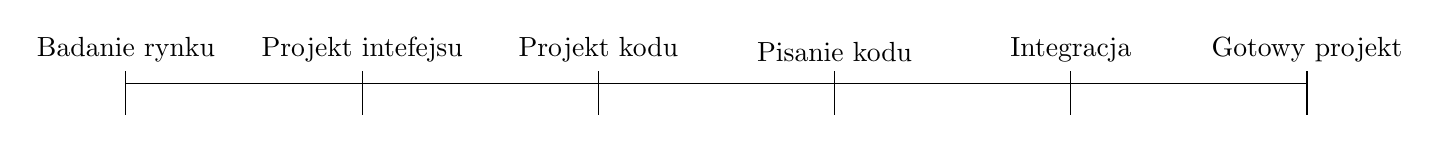
\begin{tikzpicture}
    \draw (0,0) -- (15,0);

    \foreach \x in {0,3,6,9,12,15}
    \draw (\x,0.15) -- (\x,-0.4);

    \node[anchor=south] at (0,0.15)    {Badanie rynku};
    \node[anchor=south] at (3,0.15)    {Projekt intefejsu};
    \node[anchor=south] at (6,0.15)    {Projekt kodu};
    \node[anchor=south] at (9,0.15)    {Pisanie kodu};
    \node[anchor=south] at (12,0.15)   {Integracja};
    \node[anchor=south] at (15,0.15)   {Gotowy projekt};

\end{tikzpicture}
\end{document}